
\documentclass[a4paper,12pt]{article}

\usepackage{graphicx} % Required for inserting images
\usepackage{amsmath,amssymb,amsfonts}
\usepackage{subcaption}
% -----------------------
% Package Imports
% -----------------------

% Set page margins
\usepackage[a4paper, top=1in, bottom=0.8in, left=1.1in, right=0.8in]{geometry}

% Use Times New Roman font
\usepackage{times}

% Add page numbering
\pagestyle{plain}

% Enable graphics inclusion
\usepackage{graphicx}
\usepackage{float}
% Enable code listings
\usepackage{listings}
\usepackage{xcolor} % For customizing code colors
\setlength{\parindent}{0pt}
 \usepackage{multirow}



\begin{document}
	\section{Experiment No. 2}
	
	\section{Experiment Title }
Observation of Characteristics of a Synchronous Generator.
	
	\section{Objective}
	
	The objectives of this lab are as follows:
	\begin{itemize}
		\item To analysis terminal voltage and field current.
		\item To analysis terminal voltage and rotation.
		\item To understand the generator’s excitation and performance behavior.
		
			
	\end{itemize}
	
	\section{Theory}

	
	A synchronous generator converts mechanical energy into electrical energy at a constant frequency. It operates based on the principle that the generated electrical frequency is synchronized with the mechanical speed of the rotor.
	
	The induced electromotive force (EMF) depends on the rotor speed ($S$) and the magnetic flux per pole ($\Phi$), and is expressed as:
	\[
	E \propto S \cdot \Phi
	\]
	
	Since the flux $\Phi$ is directly proportional to the field current ($I_f$), increasing the field current enhances the magnetic field strength and thus increases the terminal voltage:
	\[
	I_f \propto \Phi
	\]
	\[
	E \propto \Phi
	\]
	Thus \[
	E \propto I_f
	\]
	The synchronous speed ($S$) of the generator is related to the electrical frequency ($f$) and the number of poles ($P$) as:
	\[
	S = \frac{120f}{P}
	\]
	where $S$ is in revolutions per minute (rpm), and $f$ is in hertz (Hz).
	
	In operation, the rotor is excited with a direct current (DC) to produce a magnetic field. This rotating field induces an alternating voltage in the stator windings due to Faraday's law of electromagnetic induction. Under no-load conditions, the induced EMF per phase is given by:
	\[
	E = 4.44 f N \Phi
	\]
	where $E$ is the RMS value of the induced EMF, $f$ is the frequency, $N$ is the number of turns per phase, and $\Phi$ is the flux per pole.
	
	The relationship between terminal voltage and field current under no-load is illustrated by the Characteristic curve. As field current increases, the terminal voltage also increases, provided the speed remains constant. Additionally, increasing the speed of the prime mover raises the EMF and hence the terminal voltage.
	\section{Circuit Diagram}
		\begin{figure}[H]
		\centering
		\begin{subfigure}[t]{.9\textwidth}
			\centering
			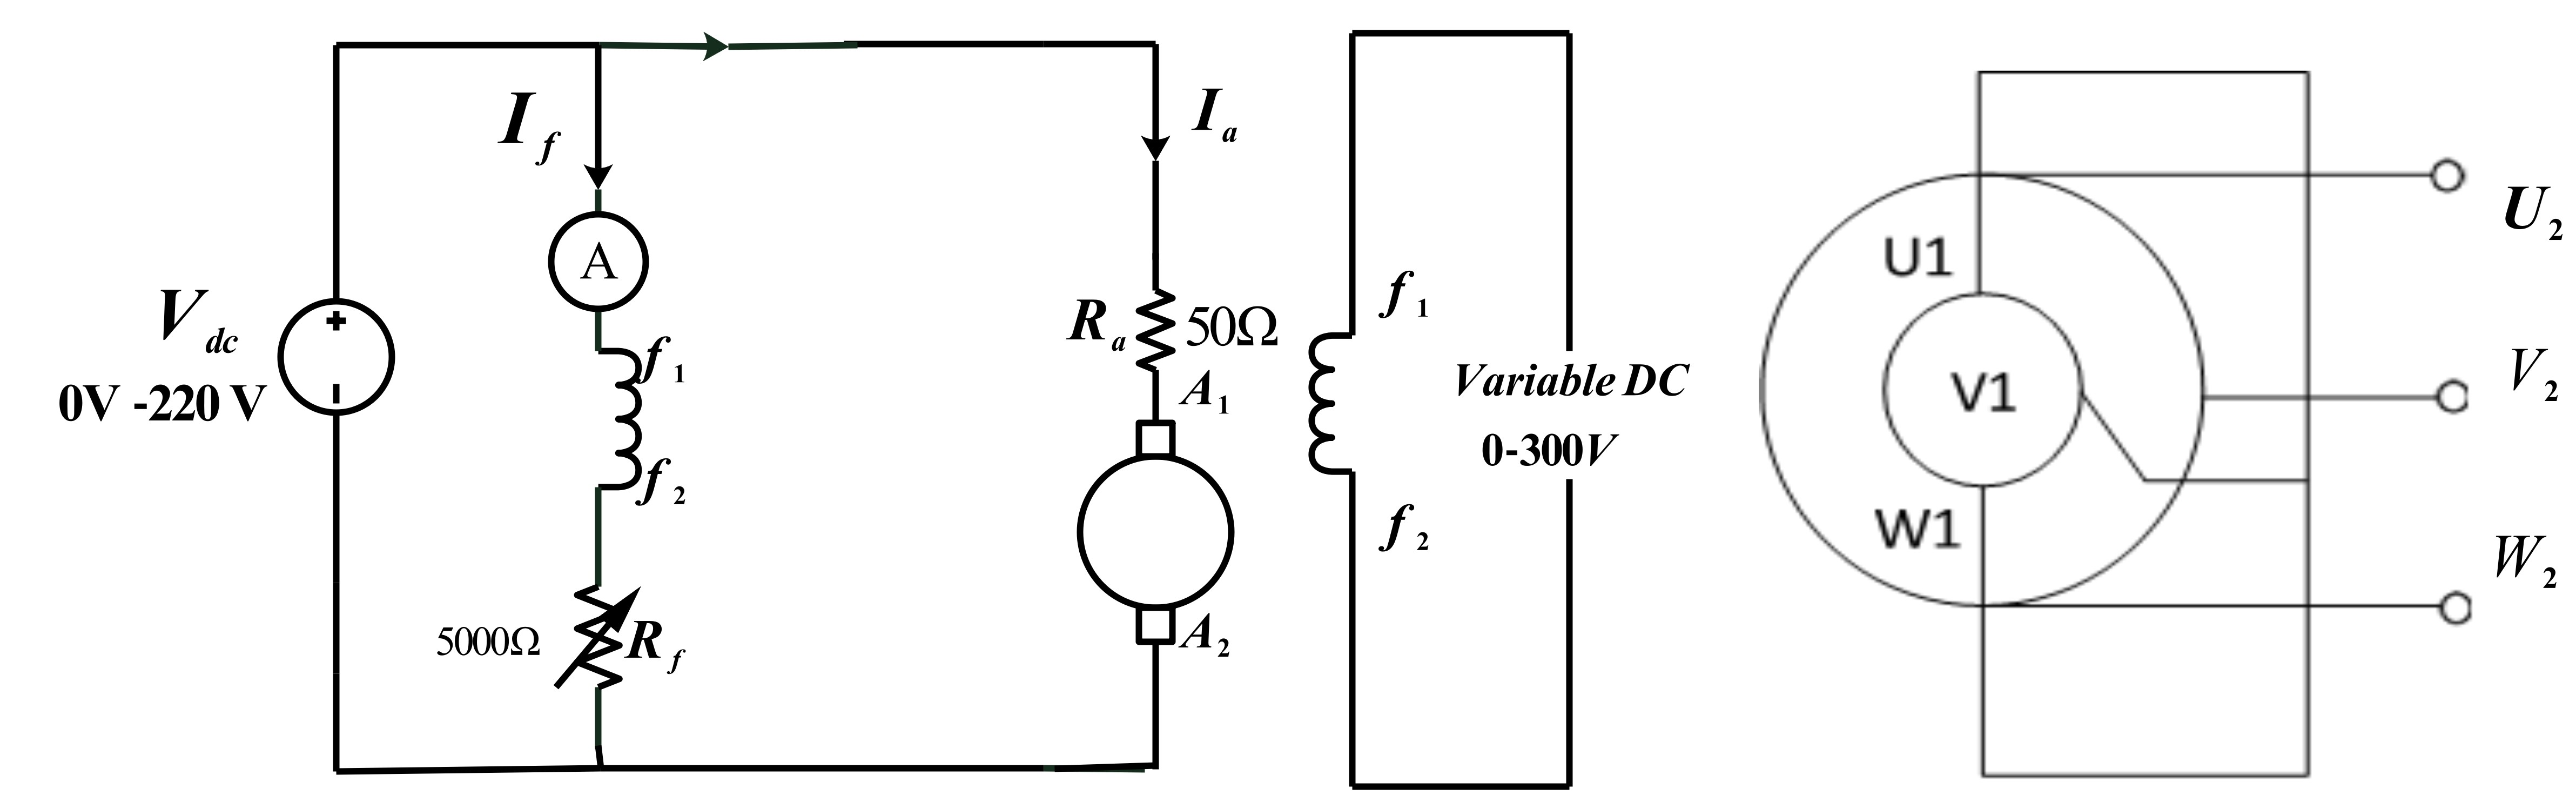
\includegraphics[width=1.1\textwidth]{Images/3108exp02}
			\caption{Circuit Diagram of Synchronus Generator.}
		
		\end{subfigure}
		
	
		
		\end{figure}
	
	\section{Required Apparatus}
	\begin{enumerate}
		\item \textbf{DC Motor}
		\begin{enumerate}
			\item Power: 300W , Speed: 3000 rpm
			\item Voltage: 220V
			\item \textbf{Excitation (Series)}: D1-D2, Current: 1.9A, \textbf{Excitation (Separate)}: F1-F2, Current: 1.8A, Excitation Voltage: 220V, Excitation Current: 0.1A
			
		\end{enumerate}
		
		\item \textbf{Synchronous Generator}
		\begin{enumerate}
			\item Power: 350W ,Power Factor: $\cos\phi = 1$ ,Speed: 3000 rpm
		
			\item Voltage: 400V (star) / 230V (delta) ,Current: 0.7A (star) / 1.2A (delta) 
			\item Excitation Voltage: 220V ,Excitation Current: 0.45A
		
		\end{enumerate}
		
		\item \textbf{Resistors}
		\begin{enumerate}
			\item 50$\Omega$: Power = 500W, Current = 3.16A
			\item 200$\Omega$: Power = 500W, Current = 1.58A
			\item 5000$\Omega$: Power = 500W, Current = 0.31A
		\end{enumerate}
		
		\item \textbf{Tachometer}
		\begin{enumerate}
			\item For 0.6V/rev: 300V at 5000 RPM , For 2mV/rev: 10V at 5000 RPM
			\item Maximum Current: 0.07A
			\item Maximum Speed: 5000 RPM
		\end{enumerate}
		
		\item \textbf{AC Multimeter}
		\begin{enumerate}
			\item 500V AC RMS
			\item 5A
		\end{enumerate}
	\end{enumerate}
	
\section{Data Table}
	% Please add the following required packages to your document preamble:
	% \usepackage{multirow}
	\begin{table}[H]
		\centering
		\caption{Readings of Terminal Voltage $V_T$ , Field Current $I_f$ and Speed $S$}
			\begin{subtable}[t]{0.45\textwidth} 
		\begin{tabular}{|c|c|c|c|}
			\hline
			\textbf{\begin{tabular}[c]{@{}c@{}}SI \\ No.\end{tabular}} & \textbf{\begin{tabular}[c]{@{}c@{}}Terminal voltage \\ $V_g  (V)$\end{tabular}} & \textbf{\begin{tabular}[c]{@{}c@{}}Field current \\ $I_f  (A)$\end{tabular}} & \textbf{\begin{tabular}[c]{@{}c@{}}Speed\\ (rpm)\end{tabular}} \\ \hline
			1                                                          & 112.0                                                                            & 0.078                                                                        & \multirow{14}{*}{3000}                                         \\ \cline{1-3}
			2                                                          & 139.1                                                                            & 0.097                                                                        &                                                                \\ \cline{1-3}
			3                                                          & 150.8                                                                            & 0.103                                                                        &                                                                \\ \cline{1-3}
			4                                                          & 160.2                                                                            & 0.110                                                                        &                                                                \\ \cline{1-3}
			5                                                          & 178.1                                                                            & 0.120                                                                        &                                                                \\ \cline{1-3}
			6                                                          & 200.0                                                                            & 0.135                                                                        &                                                                \\ \cline{1-3}
			7                                                          & 219.1                                                                            & 0.148                                                                        &                                                                \\ \cline{1-3}
			8                                                          & 258.1                                                                            & 0.176                                                                        &                                                                \\ \cline{1-3}
			9                                                          & 269.2                                                                            & 0.182                                                                        &                                                                \\ \cline{1-3}
			10                                                         & 284.2                                                                            & 0.192                                                                        &                                                                \\ \cline{1-3}
			11                                                         & 300.5                                                                            & 0.204                                                                        &                                                                \\ \cline{1-3}
			12                                                         & 312.3                                                                            & 0.213                                                                        &                                                                \\ \cline{1-3}
			13                                                         & 372.1                                                                            & 0.267                                                                        &                                                                \\ \cline{1-3}
			14                                                         & 402.1                                                                            & 0.301                                                                        &                                                                \\ \hline
		\end{tabular}
		\caption{Readings of $V_T$ and $I_f$}
			\vspace{1cm}
	\end{subtable}

		% Sub-table (b)
		\begin{subtable}[t]{0.32\textwidth} % Adjusted width for each sub-table
			\centering
			\begin{tabular}{|c|c|c|}
			\hline
			\textbf{\begin{tabular}[c]{@{}c@{}}SI \\ No.\end{tabular}} & \textbf{\begin{tabular}[c]{@{}c@{}}Terminal voltage, \\ $V_g  (V)$\end{tabular}} & \textbf{\begin{tabular}[c]{@{}c@{}}Speed\\    S (rpm)\end{tabular}} \\ \hline
			1                                                          & 400.1                                                                            & 3035                                                                \\ \hline
			2                                                          & 398.1                                                                            & 3020                                                                \\ \hline
			3                                                          & 395.4                                                                            & 3003                                                                \\ \hline
			4                                                          & 391.9                                                                            & 2976                                                                \\ \hline
			5                                                          & 390.1                                                                            & 2963                                                                \\ \hline
			6                                                          & 388.9                                                                            & 2956                                                                \\ \hline
			7                                                          & 386.7                                                                            & 2937                                                                \\ \hline
			8                                                          & 383.2                                                                            & 2915                                                                \\ \hline
			9                                                          & 380.7                                                                            & 2899                                                                \\ \hline
			10                                                         & 377.6                                                                            & 2874                                                                \\ \hline
			11                                                         & 374.2                                                                            & 2856                                                                \\ \hline
			12                                                         & 371.4                                                                            & 2835                                                                \\ \hline
			13                                                         & 363.1                                                                            & 2773                                                                \\ \hline
			14                                                         & 344.8                                                                            & 2642                                                                \\ \hline
		\end{tabular}
			\caption{Readings of $V_T$ and $S$ } % Sub-table (b) caption
		\end{subtable}
	\end{table}
\section{Graph}
	\begin{figure}[H]
	\centering
	\begin{subfigure}[t]{1\textwidth}
		\centering
		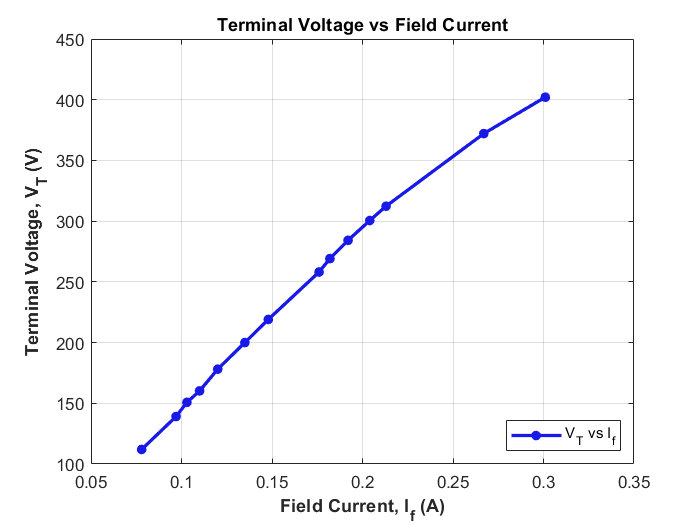
\includegraphics[width=.94\linewidth]{Images/1}
		\caption{$V_T$ vs $I_f$ Graph }
	
	\end{subfigure}
	
	\begin{subfigure}[t]{1\textwidth}
		\centering
		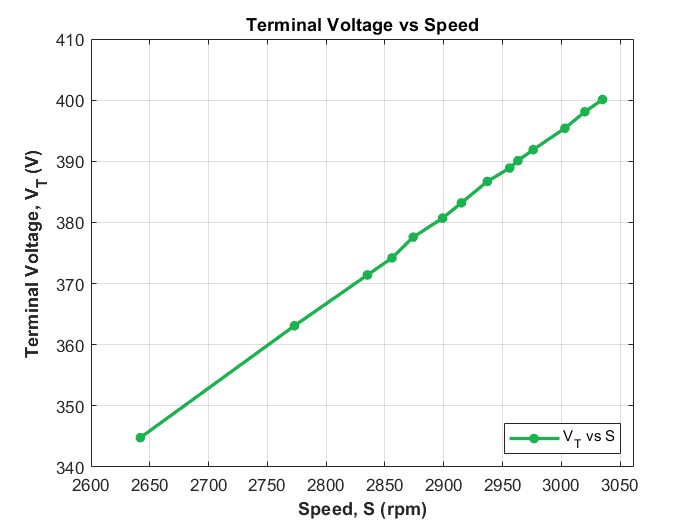
\includegraphics[width=.94\linewidth]{Images/2}
		\caption{ $V_T$ vs $S$ Graph}
	\end{subfigure}
	
	
\end{figure}
	

\section{Discussion}

The synchronous reactance of the synchronous generator was determined through Open Circuit and Short Circuit tests by varying the field current. During the Open Circuit Test, the terminal voltage increased with increasing field current, exhibiting an approximately linear relationship in the unsaturated region of the magnetic core. This behavior follows the theoretical Open Circuit Characteristic (OCC) of a synchronous generator, confirming that:

\[
E_{oc} \propto I_f
\]

In the Short Circuit Test, the short circuit current also increased linearly with the field current, as there is minimal magnetic saturation due to the low voltage during the test. 

By taking the ratio of the open-circuit voltage to the short-circuit current for corresponding field currents, the synchronous reactance ($X_s$) was estimated using the relation:

\[
X_s = \frac{V_{oc}}{I_{sc}}
\]

This value provides a measure of the internal impedance due to armature reaction and leakage reactance in the generator. The experimental data followed the expected theoretical trend, validating the method used and highlighting the dependence of $X_s$ on both excitation and the magnetic characteristics of the generator.

Overall, the experiment successfully demonstrated the process for determining synchronous reactance, an essential parameter for performance analysis and design of synchronous machines.

	
\end{document}
